\themaO
\graphicspath{{../../S28_Le_ratio/Images/}}

\chapter{Le ratio}
\label{S28}


%%%%%%%%%%%%%%%%%%%%%%%%%%%%%%%%%%%%%%%%%%
%%%%%%%%%%%%%%%%%%%%%%%%%%%%%%%%%%%%%%%%%%
\begin{prerequis}
   \begin{itemize}
      \item Notion de ratio.
      \item[\com] Partager une quantité (par exemple une somme d’argent) en deux ou trois parts selon un ratio donné.
   \end{itemize}
\end{prerequis}

\vfill

\begin{debat}[Débat : d'où vient le ratio ?] 
   {\bf Ratio} vient de l’anglais {\bf ratio} que l’on traduit par proportion qui lui-même vient du latin {\bf ratio} qui signifie calcul ou compte. Ce vocabulaire est plutôt utilisé dans le monde anglo-saxon. \\
   On le retrouve pour la première fois dans {\it Les éléments}, d'{\it Euclide}, soit il y a environ 2\,300 ans !
   \begin{center}
       \begin{pspicture}(0,0)(7.5,4.7)
         {\psset{unit=0.35}
         \psgrid[subgriddiv=0,gridcolor=lightgray,gridlabels=0pt](0,0)(21,13)
          \psframe(0,0)(21,13)
          \psline(8,0)(8,13)
          \psline(0,8)(8,8)
          \psline(5,8)(5,13)
          \psline(5,10)(8,10)
          \psline(6,8)(6,10)
          \psline(5,9)(6,9)
          \psset{linecolor=B1,linewidth=0.2}
          \psarc(8,13){13}{-90}{0}
          \psarc(8,8){8}{180}{-90}
          \psarc(5,8){5}{90}{180}
          \psarc(5,10){3}{0}{90}
          \psarc(6,10){2}{-90}{0}
          \psarc(6,9){1}{90}{-90}}
      \end{pspicture}
   \end{center}
   \bigskip
   \begin{cadre}[B2][F4]
      \begin{center}
         Vidéo : \href{https://www.youtube.com/watch?v=vDZje8o_eD4}{\bf Quel est le point commun entre un ananas, des lapins et la tour de Pise ?}, chaîne YouTube {\it Unisciel}.
      \end{center}
   \end{cadre}  
\end{debat}

\vfill

\textcolor{PartieGeometrie}{\sffamily\bfseries Cahier de compétences} : chapitre 5, exercices 36 à 46 ; 51 ; 52.


%%%%%%%%%%%%%%%%%%%%%%%%%%%%%%%%%%%%%%%%%%
%%%%%%%%%%%%%%%%%%%%%%%%%%%%%%%%%%%%%%%%%%
\activites

\begin{activite}[Représenter des ratios]
   {\bf Objectifs} :  calculer un ratio ; partager une quantité en deux ou trois parts selon un ratio donné.
   \begin{QCM}
      \begin{minipage}{7cm}
         {\psset{unit=0.8}
         \begin{pspicture}(-0.5,-0.5)(8,4)
            \psline(0,3)(0,0)(8,0)(8,3)
            \pscircle(1,0.5){0.5}
            \pscircle[fillstyle=solid,fillcolor=lightgray](2,0.5){0.5}
            \pscircle[fillstyle=solid,fillcolor=lightgray](3,0.5){0.5}
            \pscircle(4.5,0.5){0.5}
            \pscircle(5.5,0.5){0.5}
            \pscircle[fillstyle=solid,fillcolor=black](7,0.5){0.5}
            \pscircle(0.5,1.4){0.5}
            \pscircle[fillstyle=solid,fillcolor=lightgray](1.5,1.4){0.5}
            \pscircle(2.5,1.4){0.5}
            \pscircle(3.75,1.2){0.5}
            \pscircle[fillstyle=solid,fillcolor=black](5,1.4){0.5}
            \pscircle[fillstyle=solid,fillcolor=lightgray](6.25,1.2){0.5}
            \pscircle(7.5,1.4){0.5}
            \pscircle[fillstyle=solid,fillcolor=black](2,2.3){0.5}
            \pscircle(3.25,2.1){0.5}
            \pscircle[fillstyle=solid,fillcolor=lightgray](4.25,2.1){0.5}
            \pscircle(5.75,2.1){0.5}
            \pscircle(6.75,2.1){0.5}
            \pscircle[fillstyle=solid,fillcolor=black](5,2.8){0.5}
            \pscircle[fillstyle=solid,fillcolor=lightgray](3.75,3){0.5}
         \end{pspicture}}
      \end{minipage}
      \qquad
      \begin{minipage}{8cm}
         Dans cette boite, il y a 4 balles noires pour 6 balles grises. On dit que la quantité de balles noires et grises est dans le ratio de 4 : 6 (on lit \og 4 pour 6 \fg{}) ou encore 2 : 3 (\og 2 pour 3 \fg{}). \\
   Inversement, le ratio des balles grises et noires est de 6 : 4.
      \end{minipage}
      \begin{enumerate}
      \item 
      \begin{enumerate}
         \item Quel est le ratio des balles noires et blanches ? Simplifier éventuellement ce ratio. \\ [2mm]
            \pf \smallskip
         \item Quel est le ratio des balles grises et blanches ? Simplifier éventuellement ce ratio. \\ [2mm]
            \pf \smallskip
         \item Comment pourrait-on écrire le ratio de balles noires, grises et blanches ? \\ [2mm]
            \pf \smallskip
         \item Quelle fraction du total des balles représente les balles noires ? Les balles grises ? Les balles blanches ? \\ [2mm]
            \pf \smallskip
      \end{enumerate}
      \item Dans cette question, on garde les mêmes ratios que dans les questions précédentes.
      \begin{enumerate}
         \item Si le bac contenait 40 balles, combien aurait-on de balles noires ? Grises ? Blanches ? \\ [2mm]
            \pf \\ \smallskip
            Quelle fraction du total des balles représente chaque sorte de balles ? \\ [2mm]
            \pf \smallskip
         \item Si le bac contenait 10 balles, combien aurait-on de balles noires ? Grises ? Blanches ? \\ [2mm]
            \pf \\ \smallskip
            Quelle fraction du total des balles représente chaque sorte de balles ? \\ [2mm]
            \pf \smallskip
         \item Si le bac contenait 130 balles, combien aurait-on de balles noires ? Grises ? Blanches ? \\ [2mm]
            \pf \\ \smallskip
            Quelle fraction du total des balles représente chaque sorte de balles ? \\ [2mm]
            \pf \smallskip
      \end{enumerate}
      \item On souhaite partager 21 balles roses et violettes dans le ratio 3 : 4. Combien aura-t-on de balles roses et violettes ? \\ [3mm]
         \pf \smallskip
     \item On partage 48 balles bleues, blanches et rouges dans le ratio 1 : 2 : 3. Combien a-t-on de balles de chaque couleur ? \\ [2mm]
         \pf \\ \smallskip
      \end{enumerate}
   \end{QCM}
\end{activite}


%%%%%%%%%%%%%%%%%%%%%%%%%%%%%%%%%%%%%%%%%%
%%%%%%%%%%%%%%%%%%%%%%%%%%%%%%%%%%%%%%%%%%
\cours 

\section{Définition du ratio} %%%

\begin{definition}
   \psset{unit=0.75,subgriddiv=0,gridlabels=0,fillstyle=solid}
   \begin{itemize}
      \item On dit que {\bf deux nombres} $a$ et $b$ sont, par exemple, dans le {\bf ratio} 3 : 4 si $\dfrac{a}{3} =\dfrac{b}{4}$. \\
      On parle de ratio \og trois pour quatre \fg. \\
      On peut modéliser ainsi :
      \begin{pspicture}(-0.3,0)(7,1.2)
         \psframe[fillcolor=A2](0,0)(3,1)
         \psbrace[nodesepA=-0.8mm,nodesepB=3mm,rot=90](0,0)(3,0){$a$}
         \psframe[fillcolor=B2](3,0)(7,1)
         \psbrace[nodesepA=-0.8mm,nodesepB=3mm,rot=90](3,0)(7,0){$b$}
         \psgrid(0,0)(7,1)
      \end{pspicture} \\ [3mm]
      \item On dit que {\bf trois nombres} $a$, $b$ et $c$ sont, par exemple, dans le {\bf ratio} 1 : 3 : 6 si $\dfrac{a}{1} =\dfrac{b}{3} = \dfrac{c}{6}$. \\
      On parle de ratio \og un pour trois pour six \fg. \\
      On peut modéliser ainsi :
      \begin{pspicture}(-0.3,0)(7,1.2)
         \psframe[fillcolor=A2](0,0)(1,1)
         \psbrace[nodesepA=-0.8mm,nodesepB=3mm,rot=90](0,0)(1,0){$a$}
         \psframe[fillcolor=B2](1,0)(4,1)
         \psbrace[nodesepA=-0.8mm,nodesepB=3mm,rot=90](1,0)(4,0){$b$}
         \psframe[fillcolor=H2](4,0)(10,1)
         \psbrace[nodesepA=-0.8mm,nodesepB=3mm,rot=90](4,0)(10,0){$c$}
         \psgrid(0,0)(10,1)
      \end{pspicture} \\ [1mm]
   \end{itemize}
\end{definition}

\begin{exemple*1}
   Yassine et Nisrine se partagent des cookies dans un ratio 3 : 4, cela veut dire que, à chaque fois que Yassine a 3 cookies, Nisrine en a 4 si bien que le nombre de cookies que possède Yassine divisé par 3 est toujours égal au nombre de cookies que possède Nisrine divisé par 4.
\end{exemple*1}

\begin{remarque}
   attention à ne pas confondre les notations 3 : 4 ; $3\div4$ et $\dfrac34$, la première désigne un ratio, la deuxième une division et la troisième une fraction. \\
   Dans l'exemple, Yassine possède $\dfrac37$ des cookies et Nesrine $\dfrac47$. \\ [1mm]
   Chacune de ces fractions permet de comparer une partie à la totalité, ce ne sont pas des ratios.
\end{remarque}


%%%%%%%%%%%%%%%%%%%%%%%
\section{Méthode de partage suivant un ratio}

\begin{methode}
Pour partager une quantité suivant un ratio :
   \begin{itemize}
      \item on calcule le nombre de parts égales à distribuer en additionnant les nombres du ratio ;
      \item on divise la quantité par le nombre de parts à distribuer ce qui nous donne la quantité par part ;
      \item on distribue les parts selon le ratio.
   \end{itemize}
   \exercice
   On souhaite partager 15 pièces d'or entre les pirates Seyon et Lloyd suivant le ratio 2 : 3. \\
   Combien vont-ils avoir de pièces d'or chacun ?
   \correction
   \ \\ [-10mm]
   \begin{itemize}
      \item Les 15 pièces d'or sont partagées en 5 parts égales (2 parts pour Seyon et 3 parts pour Lloyd).
      \item $15\text{ pièces d'or}\div 5 =3\text{ pièces d'or}$ donc, une part vaut 3 pièces d'or.
     \item Seyon a 2 parts, soit $2\times3\text{ pièces d'or} =6\text{ pièces d'or}$ et Lloyd a 3 parts, soit $3\times3\text{ pièces d'or} =9\text{ pièces d'or}$. 
   \end{itemize}
   On peut également dire que Seyon et Lloyd se partagent les pièces d'or suivant le ratio 6 : 9.
\end{methode}


%%%%%%%%%%%%%%%%%%%%%%%%%%%%%%%%%%%%%%%%%%
\exercicesbase

\begin{colonne*exercice}

%%%%%%%%%%%%%%%
\serie{Calculer un ratio} %%%

\smallskip

\begin{exercice} %1
   Simplifier les ratios suivants.
   \begin{colenumerate}{3}
      \item 35 : 20
      \item 49 : 70
      \item18 : 24
   \end{colenumerate}
\end{exercice}

\begin{corrige}
   \ \\ [-5mm]
   \begin{enumerate}
      \item On simplifie par 5 et on obtient {\blue 7 : 4}
      \item On simplifie par 7 et on obtient {\blue 7 : 10}
      \item On simplifie par 6 et on obtient {\blue 3 : 4}
   \end{enumerate}
\end{corrige}

\bigskip


\begin{exercice} %2
   Déterminer des ratios.
   \begin{enumerate}
      \item Un paquet de bonbons contient 13 bonbons à la fraise et 8 au citron. \\
         Dans quel ratio sont les bonbons à la fraise et les bonbons au citron ?
      \item Un paquet de bonbons contient 28 bonbons à la fraise, 18 au citron et 14 au cola. \\
         Dans quel ratio sont les bonbons à la fraise, les bonbons au citron et les bonbons au cola ?
   \end{enumerate}
\end{exercice}

\begin{corrige}
   \ \\ [-5mm]
   \begin{enumerate}
      \item Les bonbons à la fraise et au citron sont dans le ratio {\blue 13 : 8}
      \item Les bonbons à la fraise, au citron et au cola sont dans le ratio {\blue 28 : 18 : 14} ou encore 14 : 9 : 7
   \end{enumerate}
\end{corrige}

\bigskip


\begin{exercice} %3
   Utiliser le dessin ci-dessous pour répondre aux questions.
   \begin{center}
   \psset{unit=0.9,subgriddiv=0,gridlabels=0,fillstyle=solid}
      \begin{pspicture}(0,0.5)(7,3)
         \def\noir{\psframe[fillcolor=black](0,0)(1,1)}
         \rput(0,0){\noir}
         \rput(0,2){\noir}
         \rput(3,0){\noir}
         \rput(3,2){\noir}
         \rput(6,0){\noir}
         \rput(6,2){\noir}
         \psframe[fillcolor=B2](1,1)(3,2)
         \psframe[fillcolor=B2](4,1)(6,2)
         \psgrid(0,0)(7,3)
      \end{pspicture}
   \end{center}
   \begin{enumerate}
      \item Quel est le ratio carrés rouges - total de carré ?
      \item Que peut représenter le ratio 4 : 6 ?
      \item Selon quel ratio sont représentés les carrés noirs et les carrés blancs ?
   \end{enumerate}
\end{exercice}

\begin{corrige} 
   \ \\ [-5mm]
   \begin{enumerate}
      \item Le ratio carrés rouges - total de carré est {\blue 4 : 21}
      \item 4 : 6 peut représenter le {\blue ratio des carrés rouges et} {\blue des carrés noirs.}
      \item Les carrés noirs et les carrés blancs sont dans le ratio {\blue 6 : 11}
   \end{enumerate}
\end{corrige}

\bigskip


\begin{exercice} %4
   Utiliser ce tableau des matchs perdus ou gagnés d'un collège pour répondre aux questions.
   \begin{center}
      {\hautab{1.25}
      \begin{CLtableau}{0.9\linewidth}{4}{c}
         \hline
         Sport & matchs gagnés & matchs perdus \\
         \hline
         Rugby & 9 & 6 \\
         \hline
         Judo & 12 & 8 \\
         \hline
         Handball & 10 & 5 \\
         \hline
      \end{CLtableau}}
   \end{center}
   \begin{enumerate}
      \item Quels sports ont un ratio équivalent gains-pertes ?
      \item Pour le handball :
      \begin{enumerate}
         \item Quel est le ratio gains-matchs joués ?
         \item Quelle est la fraction de matchs gagnés ?
         \item Quel est le pourcentage de matchs gagnés ?
      \end{enumerate}
   \end{enumerate}
\end{exercice}

\begin{corrige}
  \ \\ [-5mm]
  \begin{enumerate}
      \item Rugby : ratio gains - pertes de 9 : 6 $=$ 3 : 2 \\
      Judo : ratio gains - pertes de 12 : 8 $=$ 3 : 2 \\
      Handball : ratio gains - pertes de 10 : 5 $=$ 2 : 1 \\
      {\blue Le rugby et le judo ont le même ratio gains - pertes.}
      \item 
      \begin{enumerate}
         \item Pour le handball, le ratio gains - matchs joués est de 10 : 15 équivalent à {\blue 2 : 3} \\
         \item La fraction de matchs gagnés est de $\dfrac{10}{15} = \blue \dfrac23$ \\ [1mm]
         \item Le pourcentage de matchs gagnés est de $\dfrac{10}{15}\times100 \approx {\blue 67\,\%}$
      \end{enumerate}
   \end{enumerate}
\end{corrige}

\bigskip


\serie{Calculer des quantité grâce à un ratio} %%%

\smallskip

\begin{exercice} %5
   Quelle quantité d'huile et de vinaigre utilise-t-on dans une vinaigrette de \uml{500} réalisée dans le ratio 3~:~1 ?
\end{exercice}

\begin{corrige}
   Le ratio 3 : 1 pour l'huile est le vinaigre signifie que pour \uml{3} d'huile, on doit mettre \uml{1} de vinaigre pour un total de \uml{4} de vinaigrette. \\
   Si on souhaite \uml{500} de vinaigrette, il faut multiplier les quantités par 125 ($500\div4=125$). \\
   Il faut donc {\blue \uml{375} d'huile pour \uml{125} de vinaigre.} \medskip
\end{corrige}

\bigskip


\begin{exercice} %6
   Deux amis ont joué au loto et leur mise s'est faite selon le ratio 3 : 5. Ils gagnent \ueuro{64}. \\
   Quelle est la somme d'argent qui revient à chacun d'eux ?
\end{exercice}

\begin{corrige}
   Le ratio 3 : 5 signifie que lorsqu'un joueur gagne \ueuro{3}, l'autre gagne \ueuro{5} pour une somme de \ueuro{8}. \\
   S'ils gagnent \ueuro{64}, c'est-à-dire 8 fois plus, {\blue l'un gagnera \ueuro{24} et l'autre \ueuro{40}.} \medskip
\end{corrige}

\bigskip


\begin{exercice} %7
   Une recette de biscuits sablés commence par la fabrication d'un \og sable \fg{} réalisé avec de la farine, du beurre et du sucre dans le ratio 10 : 6 : 5. Une pâte homogène est ensuite fabriquée avec ce sable et un peu de lait. \\
   Quelles masses de farine, de beurre et de sucre doit-on prendre pour créer un \og sable \fg{} de \ug{630} ?
\end{exercice}

\begin{corrige}
   Le ratio 10 : 6 : 5 signifie que pour \ug{21} de pâte, on a \ug{10} de farine, \ug{6} de beurre et \ug{5} de sucre. \\
   Donc, pour \ug{630} de pâte, c'est-à-dire 30 fois plus ($630\div21=30$), on aura {\blue \ug{300} de farine, \ug{180} de beurre et \ug{150} de sucre.} \medskip
\end{corrige}

\bigskip


\begin{exercice} %8
   Pour récompenser leurs enfants Clémentine, Myrtille et Prune, qui les ont beaucoup aidés, M. et Mme Potager leur donnent un peu d'argent. Ils leur distribuent \ueuro{120} selon le ratio 3 : 4 : 5 parce qu'ils n'ont pas aidé autant les uns que les autres. \\
   Combien chacun va-t-il recevoir ?
\end{exercice}

\begin{corrige}
   Le ratio 3 : 4 : 5 signifie que Clémentine reçoit \ueuro{3} lorsque Myrtille reçoit \ueuro{4} et Prune \ueuro{5} pour un total distribué de \ueuro{12}. Pour \ueuro{120}, c'est-à-dire 10 fois plus, {\blue Clémentine aura \ueuro{30}, Myrtille \ueuro{40} et Prune \ueuro{50}}. \medskip
\end{corrige}

\bigskip


\begin{exercice} %9
   Dans une assemblée, le ratio hommes-femmes est de 50 : 45. \\
   Si cinq femmes entrent, le ratio sera-t-il de 50 : 50 ?
\end{exercice}

\begin{corrige}
   Un ratio hommes-femmes de 50 : 45 signifie que pour 50 hommes, il y a 45 femmes. \\
   Imaginons une assemblée de 500 hommes et 450 femmes (10 fois plus), si cinq femmes entrent, on aura 500 hommes pour 455 femmes donc un ratio de 500~:~455 ce qui n'est {\blue pas équivalent à un ratio de 50 : 50.} \medskip
\end{corrige}

\bigskip


\begin{exercice} %10
   Adam va fêter ses 13 ans. Avant son anniversaire, il essaie une nouvelle recette de cocktail sans alcool, pour laquelle il faut 2 verres de jus d'orange pour 3 verres de jus d'ananas et 4 verres de jus de pomme. \\
   Cette recette lui plaît. Pour tous ses amis, il veut préparer \ul{45} de cocktail. \\
   Combien de litres de chaque ingrédient doit-il acheter ?
   \begin{center}
      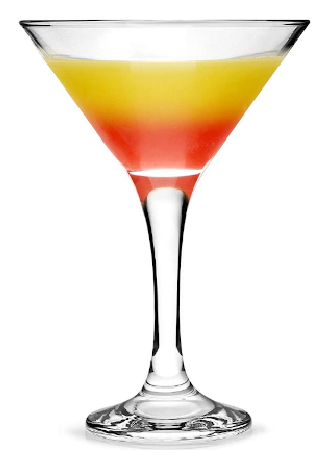
\includegraphics[width=1.3cm]{coktail}
   \end{center}
\end{exercice}

\begin{corrige}
   Le jus d'orange, d'ananas et de pomme sont dans le ratio 2 : 3 : 4. Donc, pour \ul{2} de jus d'orange, il faut \ul{3} de jus d'ananas et \ul{4} de jus de pomme ce qui donne \ul{9} de cocktail. \\
   Pour \ul{45}, soit 5 fois plus, il faut {\blue \ul{10} de jus d'orange, \ul{15} de jus d'ananas et \ul{20} de jus de pomme}.
   
\bigskip
\corec{The golden ratio}
\smallskip

\begin{enumerate}
   \item Cette question est personnelle, cependant, {\blue le rectangle d} semble être le plus équilibré.
   \item Tableau complété : \\ \smallskip
   {\hautab{1.2}
      \small
      \begin{CLtableau}{\linewidth}{6}{c}
         \hline
         Rectangle & a & b & c & d & e \\
         \hline
         Length ($\ell$) in \ucm{} & 2 & 4 & 6 & 4 & 9 \\
         \hline
         Width ($w$) in \ucm{} & 2 & 2,5 & 2 & 2 & 1 \\
         \hline
         $\ell\div w$ & 1 & 1,6 & 3 & 2 & 9 \\
         \hline
      \end{CLtableau}}
   \item {\blue $10\div6,18 \approx 1,618$} et {\blue $6,18\div3,82 \approx 1,618$}.
   \item On trouve les dénominations suivantes : \\ 
      {\blue THE GOLDEN RATIO} ; \\
      {\blue THE GOLDEN PROPORTION} ; \\
      {\blue THE DIVINE PROPORTION} ; \\
      {\blue THE GOLDEN NUMBER}. \smallskip
   \item $\phi =\dfrac{1+\sqrt5}{2} \approx {\blue 1,618}$.
\end{enumerate}


\end{corrige}


\vfill\hfill\footnotesize{D'après \href{https://ent2d.ac-bordeaux.fr/disciplines/mathematiques/les-ratios-au-college/}{\og Les ratios au collège \fg{}}, académie de Bordeaux.}

\end{colonne*exercice}


%%%%%%%%%%%%%%%%%%%%%%%%%%%%%%%%%%%%%%%%%%
\Recreation

\enigme[The golden ratio]
 
\begin{enumerate}
   \item Among the following rectangles, circle the one you think is the most attractive and well-balanced.
   \begin{center}
      \begin{pspicture}(0,0)(14,5.5)
         \psset{fillstyle=solid}
         \psframe[fillcolor=A3](0,0)(2,2)
         \rput(1,1){a}
         \psframe[fillcolor=C3](3,0)(7,2.47)
         \rput(5,1.235){b}
         \psframe[fillcolor=G3](8,0)(14,2)
         \rput(11,1){c}
         \psframe[fillcolor=J3](0,3)(4,5)
         \rput(2,4){d}
         \psframe[fillcolor=D3](5,3)(14,4)
         \rput(9.5,3.5){e}
      \end{pspicture}
   \end{center}
   \item Measure each rectangle's length and width, and compare the ratio of length to width for each rectangle above : \\
   \begin{center}
      \small
      {\hautab{1.5}
      \begin{CLtableau}{0.8\linewidth}{6}{c}
         \hline
         Rectangle & a & b & c & d & e \\
         \hline
         Length ($\ell$) in \ucm{} & & & & & \\
         \hline
         Width ($w$) in \ucm{} & & & & & \\
         \hline
         $\ell\div w $ & & & & & \\
         \hline
      \end{CLtableau}}
   \end{center}
   \item Draw a segment \ucm{10} long then make a small mark on it \ucm{6.18} along. Divide the length of the whole line by the length of the long section just made. Divide the length of the long section by the length of the short section. What ratios do you get? \\ [1cm]
   \item Unscramble the words to find out the various names of this ratio. \smallskip
   \begin{center}
      \renewcommand{\arraystretch}{1.2}
      \begin{tabular}{|p{2cm}p{4cm}|p{2cm}p{4cm}|}
         \hline
         TEH & \_ \_ \_ & HET & \_ \_ \_ \\
         DEOGNL & \_ \_ \_ \_ \_ \_ & NODLEG & \_ \_ \_ \_ \_ \_ \\
         TAIRO & \_ \_ \_ \_ \_ & NOOPOITRRP & \_ \_ \_ \_ \_ \_ \_ \_ \_ \_ \\
         \hline
         ETH & \_ \_ \_ & HTE & \_ \_ \_ \\
         DIINVE & \_ \_ \_ \_ \_ \_ & DEONLG & \_ \_ \_ \_ \_ \_ \\
         TINPOORPRO & \_ \_ \_ \_ \_ \_ \_ \_ \_ \_ & NEBRUM & \_ \_ \_ \_ \_ \_ \\
         \hline
      \end{tabular}
   \end{center}
   \smallskip
   \item This number named golden ratio is $\phi =\dfrac{1+\sqrt5}{2}$. Calculate is value with your calculator : \pfb
\end{enumerate}

\vfill

\begin{minipage}{10cm}
   A golden rectangle has a length to width ratio called the golden ratio, which is approximately 1.618. It is used often in art and architecture. For example, the front of the Parthenon, a temple in Athens, Greece fits into a golden rectangle.
\end{minipage}
\qquad
\begin{minipage}{5cm}
   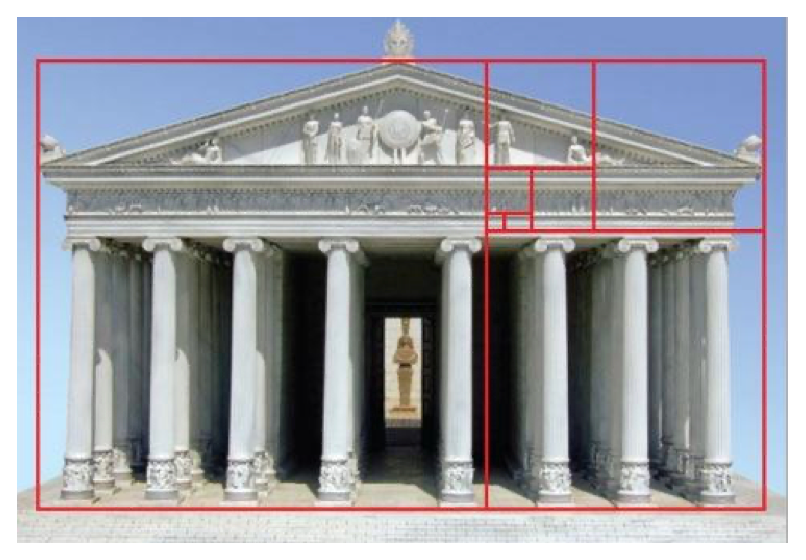
\includegraphics[width=4.5cm]{Parthenon}
\end{minipage}
   

